\documentclass[a4paper,12pt]{article}

\usepackage[russian]{babel}
\usepackage{cmap}
\usepackage[utf8]{inputenc}
\usepackage[usenames]{color}
\usepackage{tabularray}
\usepackage{xcolor}
\usepackage{graphicx} 
\usepackage{subfigure}
\usepackage{subcaption}

\usepackage[unicode]{hyperref} % цвета гиперссылок
\hypersetup{
	colorlinks,
	citecolor=black,
	filecolor=black,
	linkcolor=blue,
	urlcolor=black
}

\usepackage{geometry} % задаёт поля 
%\geometry{left=3cm}
%\geometry{right= 1.5cm}
%\geometry{top=2cm}
%\geometry{bottom=2cm} 

\usepackage{enumitem} % настраивает работу со списками:
\def\labelitemi{—} % ... задаёт длинное тире как стандартный маркер ненумерованного списка
\setlist{nolistsep} %  ... убирает дополнительный отступы между элементами списка


% удаляет названия и продолжение следует и т. для таблиц, будет только таблица без всего
\DefTblrTemplate{contfoot-text}{default}{}
\DefTblrTemplate{conthead-text}{default}{}
\DefTblrTemplate{caption}{default}{}
\DefTblrTemplate{conthead}{default}{}
\DefTblrTemplate{capcont}{default}{}


\title{Применение сингулярных разложений к обнаружению выбросов в данных о потреблении контента}
\author{В. Г. Мосин}
\date{}

%   \input{preamble.tex}
\begin{document}
	\maketitle
	\abstract{\noindent Рассмотрен метод выявления аномальных объектов, основанные на редукции данных к главным направлениям и не требующий предварительной разметки данных на нормальные и аномальные объекты. Метод реализован в виде алгоритма и протестирован на данных о потреблении контента одного из ведущих хостингов.}
	
\tableofcontents
	
\section{Введение}
Одной из важных задач анализа данных является обнаружение шума в данных и его последующее исключение для получения более надежных результатов, не зависящих от случайных флуктуаций (см. [6], [7]).

Шум в данных — это нежелательные, случайные или неточные значения, которые вносят искажения или искажают истинные данные. Шум может возникать по разным причинам, таким как ошибки измерений, неполадки в оборудовании, случайные факторы или неправильные записи. Шум может иметь различные формы и влиять на данные по-разному. Некоторые типы шума включают случайный шум, выбросы (аберрации), грубые ошибки, систематические искажения и многие другие. 

Поскольку шум может вносить искажения в данные, его наличие может затруднить анализ и интерпретацию данных. Это может привести к неправильным выводам и недостоверным результатам. Поэтому важно применять методы обработки данных и фильтрации шума для улучшения качества данных перед анализом или использованием их для принятия решений. Методы борьбы с шумом могут включать фильтрацию, сглаживание (например, сглаживание скользящим средним), применение алгоритмов обнаружения выбросов или применение статистических методов для определения и удаления шумовых значений. 

Вместе с тем, важно отметить, что в некоторых случаях шум может содержать полезную информацию или быть результатом естественных изменений в данных. Поэтому необходимо тщательно анализировать и контролировать шум, чтобы минимизировать его влияние на данные и сохранить релевантные и достоверные сведения.

\subsection{Теоретическая часть}

Обнаружение выбросов относится к предварительной обработке данных, которая, как правило, предшествует основной задаче: задаче моделирования и прогнозирования целевых признаков. Для того чтобы модели обладали лучшими характеристиками, а их прогнозы были более точными, из обучающих наборов данных важно исключать записи, являющиеся нетипичными или аномальными (см. [7]).

Это связано с тем, что обучение модели на типичных объектах позволяет ей лучше улавливать общие закономерности и характеристики в данных. Аномальные объекты могут содержать случайные или экстремальные значения, которые могут отличаться от общих трендов и снизить способность модели к обобщению на новые, неизвестные объекты.

Кроме того, аномальные объекты могут вносить существенные искажения в данные и повлиять на модель, если они включены в процесс обучения. Модель может стремиться адаптироваться к этим выбросам, в результате чего потеряется способность модели к правильному предсказанию на типичных данных.
И наконец, обучение на типичных объектах помогает создать более надежную и стабильную модель. Такие модели обычно лучше справляются с новыми данными и более точно предсказывают результаты. Тогда как модель, обученная на аномальных объектах, может быть менее надежной и неустойчивой к изменениям в данных.

Не менее важной является и задача прогнозирования (см. [6]). Обученная стабильная модель, дающая хорошие результаты на типичных объектах, вполне может оказаться непригодной при попытке спрогнозировать значения целевых признаков в ситуациях, сильно отличающихся от тех, на которых модель обучалась. 

Это проявляется, прежде всего,  в низкой точности прогнозов. Если модель не была обучена на разнообразных данных и не встречала сильно отличающиеся друг от друга примеры, ее прогноз может быть неточным на таких данных. Модель может не уловить закономерности или связи между признаками в новых данных, что приведет к плохим прогнозам.

Вдобавок к этому происходит потеря обобщающей способности. Если модель была обучена на данных с определенными характеристиками и структурой, она может не получить достаточной обобщающей способности для предсказания на данных с другой структурой или характеристиками. 
Необходимо помнить, что модель машинного обучения является результатом обучения на конкретных данных, и ее прогнозы оказываются наиболее точными в пределах набора данных, на котором она обучалась. Для этого нужно уметь различать объекты, подаваемые на вход модели для прогнозирования, нужно уметь выявлять нетипичные объекты и исключать их из процесса еще до подачи в модель.

\subsection{Постановки задачи}

Если данные, используемые для обучения модели, являются размеченными, то есть, каждый объект  обладает меткой «норма/аномалия», то задача обнаружения выбросов на обучающих данных вообще не стоит, а обнаружение выбросов на новых данных сводится к задаче бинарной классификации по признаку-метке (см. [4]).

Допустим, что изначально у нас нет никаких сведений о том, какие объекты относятся к числу типичных объектов, пригодных для обучения модели, а какие — к аномальным, то есть, тем, которые следует исключить из процесса обучения, чтобы избежать неприятностей, о которых было подробно сказано выше.

\subsubsection{Предмет исследования} Предметом нашего исследования является метод, позволяющий выявить нетипичные объекты в данных, не являющихся изначально размеченными по признаку «норма/аномалия». 

\subsubsection{Методика исследования} Метод основан на сингулярных матричных разложениях и последующей редукции данных к главным направлениям. Если редуцированные данные обладают слишком большой реконструкционной ошибкой, то такие объекты признаются аномальными. Мы применяем в качестве критерия выброса процент от общего объема обучающих данных, то есть, относим к типичным их объектам $K$-й перцентиль (где $K$ достаточно велико), а объекты, не попадающие в него, объявляем нетипичными выбросами.

\subsubsection{Цель исследования} Наша цель — получить алгоритм, индексирующий объекты обучающей выборки как аномальные по заданному перцентилю выбросов. Кроме того, мы собираемся применить этот алгоритм к новым данным, и, используя полученный на обучающей выборке порог отсечения, выделить в них нетипичные объекты.

\subsection{Библиотеки}
Для выполнения вычислений и анализа данных мы пользуемся средой \texttt{Jupyter Notebook}, которая предоставляет удобные средства для работы с языком программирования Python и его главными библиотеками: \texttt{NumPy}, \texttt{Pandas}, \texttt{sklearn} и \texttt{matplotlib}. Благодаря этим инструментам, мы можем эффективно работать с данными, выполнять исследования и визуализировать результаты (см. [1], [2]). 

%Библиотека \texttt{numpy} является одной из ключевых библиотек для научных вычислений и обработки массивов данных в языке программирования \texttt{Python}. Библиотека \texttt{pandas}~--- одна из наиболее популярных и мощных библиотек для работы с данными в языке программирования \texttt{Python} (см. [1]). 

%Библиотека \texttt{scikit-learn}, широко известная как \texttt{sklearn}, предоставляет обширный набор инструментов и функций для решения различных задач в языке программирования Python, таких как задачи классификации, регрессии, кластеризации и др. Мы используем эту библиотеку для решения регрессионных задач.

\section{Описание данных}
Используются данные о потреблении контента одного из ведущих хостингов за 500 дней: с 2021-08-20 по 2023-01-01. Объектами таблицы служат даты. Признаки описывают различные характеристики объекта: 'Просмотры', 'Время просмотра (часы)' и т. д. Полную структуру данных см. ниже, шаг 3.2 алгоритма исследования.

\section{Алгоритм}
\subsection{Чтение данных}
Методом \texttt{read\_csv} библиотеки \texttt{pandas} загружаем в среду исполнения набор данных и формируем дата-фрейм. 
\noindent
%---------------------------------------
%---------------------------------------
\SetTblrInner{rowsep=3pt}
%---------------------------------------
\begin{longtblr}
	{
		colspec = {
			X[r,f]
			X[r,f,4] 
			X[r,f,4] 
			X[r,f,4] 
			X[r,f,4]
			X[r,f,4]
		},
		width = \linewidth,
		rowhead = 1, 
		rowfoot = 0,
		row{odd} = {}, 
		row{even} = {},
		rows    = {font=\scriptsize},
		row{1}  = {font=\scriptsize\bfseries}
	}
	&
	Дата
	& 
	Просмотры
	&
	Поделились
	&
	...
	& 
	Лайки
	\\
	\hline[1pt]
	
	\textbf{0}   &2023-01-01	&475.0	&9.0	&…	&16.0
	\\
	\hline
	\textbf{1}   &2022-12-31	&174.0	&1.0	&…	&4.0
	\\
	\hline
	\textbf{2}   &2022-12-30	&490.0	&3.0	&…	&3.0
	\\
	\hline
	\textbf{...} & ...  & ...  & ...  & ... & ... 
	\\
	\hline
	\textbf{498} &2021-08-21	&222.0	&0.0	&…	&4.0
	\\
	\hline
	\textbf{499} &2021-08-20	&209.0	&0.0	&…	&1.0
	\\
	\hline[1pt]
\end{longtblr}
%---------------------------------------
\noindent
В данных присутствуют 500 объектов. В качестве индекса выступает дата, таким образом, объектами служат даты. Все признаки относятся к типу с плавающей запятой, пропущенных значений нет. 

\subsection{Разделение на train и test}

Используем модуль \texttt{model\_selection} библиотеки \texttt{sklearn}. Применяем метод \texttt{train\_test\_split} с параметром \texttt{test\_size=0.2}. Получаем два датафрейма: \texttt{df\_train} объемом 400 объектов и \texttt{df\_test} объемом 100 объектов.

\subsection{Нормализация обучающей выборки}

Применяем к обучающей выборке метод \texttt{describe} библиотеки \texttt{pandas} и получаем сведения о статистиках по всем признакам.

\noindent
%---------------------------------------
%---------------------------------------
\SetTblrInner{rowsep=3pt}
%---------------------------------------
\begin{longtblr}
	{
		colspec = {
			X[r,m, 4]
			X[r,m] 
			X[r,m] 
			X[r,m] 
			X[r,m]
		},
		width = \linewidth,
		rowhead = 1, 
		rowfoot = 0,
		row{odd} = {}, 
		row{even} = {},
		rows    = {font=\scriptsize},
		row{1}  = {font=\scriptsize\bfseries}
	}
	&
	min 
	& 
	mean
	&
	max 
	&
	std
	\\
	\hline[1pt]
	\textbf{Просмотры} 
	&159.00	&936.51	&2200.00	&418.144
	\\
	\hline
	\textbf{Время просмотра (часы)} 
    &5.48	&37.17	&96.72	    &16.64
	\\
	\hline
	\textbf{Поделились} 
    &0.00	&6.96	&71.00	&6.25
	\\
	\hline
	\textbf{Постоянные зрители} 
	&30.00	&163.34	&463.00	&78.90
	\\
	\hline
	\textbf{Новые комментарии} 
	&0.00	&0.53	&6.00	&0.83
	\\
	\hline
	\textbf{Отказались от подписки} 
	&0.00	&2.77	&29.00	&2.55
	\\
	\hline
	\textbf{Новые подписчики} 
	&0.00	&6.49	&19.00	&3.51
	\\
	\hline
	\textbf{Новые зрители} 
	&60.00	&366.83	&735.00	&174.01
	\\
	\hline
	\textbf{Среднее число просмотров одним пользователем} 
    &1.31	&1.79	&2.85	&0.21
	\\
	\hline
	\textbf{Уникальные зрители} 
	&96.00	&530.18	&1103.00	&239.22
	\\
	\hline
	\textbf{CTR для значков видео (\%)} 
	&1.25	&5.54	&8.52	&1.11
	\\
	\hline
	\textbf{Показы} 
	&1938.00	&8093.78	&39479.00	&3816.08
	\\
	\hline
	\textbf{Подписчики} 
	&0.00	&3.72	&15.00	&4.02
	\\
	\hline
	\textbf{Средний процент просмотра (\%)} 
	&18.68	&26.72	&41.29	&3.41
	\\
	\hline
	\textbf{Процент лайков} 
	&0.00	&92.02	&100.00	&10.31
	\\
	\hline
	\textbf{Средняя продолжительность просмотра} 
	&96.07	&144.33	&211.02	&15.66
	\\
	\hline
	\textbf{Дизлайки} 
	&0.00	&1.28	&10.00	&1.34
	\\
	\hline
	\textbf{Лайки} 
	&0.00	&15.80	&70.00	&9.13
	\\
	\hline[1pt]
\end{longtblr}
%---------------------------------------
\noindent
Значения некоторых признаков (например, 'Показы' и 'Среднее число просмотров одним пользователем') отличаются на порядки. Чтобы избежать дисбаланса размерностей, нормализуем данные обучающей выборки приведением к стандартному виду:

\medskip
\noindent
\texttt{~~df\_train\_norm = (df\_train – df\_train.mean())/df\_train.std()}

\medskip
\noindent 
После этого все признаки, во-первых, оказываются центрированными, то есть, обладают нулевыми средними, а во-вторых, их дисперсии становятся единичными, и дисбаланс размерностей исчезает:
\noindent
%---------------------------------------
%---------------------------------------
\SetTblrInner{rowsep=3pt}
%---------------------------------------
\begin{longtblr}
	{
		colspec = {
			X[r,m, 4]
			X[r,m] 
			X[r,m] 
			X[r,m] 
			X[r,m]
		},
		width = \linewidth,
		rowhead = 1, 
		rowfoot = 0,
		row{odd} = {}, 
		row{even} = {},
		rows    = {font=\scriptsize},
		row{1}  = {font=\scriptsize\bfseries}
	}
	&
	min 
	& 
	mean
	&
	max 
	&
	std
	\\
	\hline[1pt]
	\textbf{Просмотры} 
	&--1.85	&0.00	&3.02	&1.00
	\\
	\hline
	\textbf{Время просмотра (часы)} 
	&--1.90	 &0.00	&3.57	&1.00
	\\
	\hline
	\textbf{Поделились} 
	*--1.11	&0.00	&10.23	&1.00
	\\
	\hline
	\textbf{Постоянные зрители} 
	&--1.69	&0.00	&3.79	&1.00
	\\
	\hline
	\textbf{Новые комментарии} 
	&--0.64	&0.00	&6.57	&1.00
	\\
	\hline
	\textbf{Отказались от подписки} 
	&--1.08	&0.00	&10.27	&1.00
	\\
	\hline
	\textbf{Новые подписчики} 
    &--1.84	&0.00	&3.55	&1.00
	\\
	\hline
	\textbf{Новые зрители} 
	&--1.76	&0.00	&2.11	&1.00
	\\
	\hline
	\textbf{Среднее число просмотров одним пользователем} 
	&--2.23	&0.00	&4.92	&1.00
	\\
	\hline
	\textbf{Уникальные зрители} 
    &--1.81	&0.00	&2.39	&1.00
	\\
	\hline
	\textbf{CTR для значков видео (\%)} 
	&--3.84	&0.00	&2.67	&1.00
	\\
	\hline
	\textbf{Показы} 
	&--1.61	&0.00	&8.22	&1.00
	\\
	\hline
	\textbf{Подписчики} 
	&--6.63	&0.00	&2.80	&1.00
	\\
	\hline
	\textbf{Средний процент просмотра (\%)} 
	&--2.35	&0.00	&4.26	&1.00
	\\
	\hline
	\textbf{Процент лайков} 
	&--8.92	&0.00	&0.77	&1.00
	\\
	\hline
	\textbf{Средняя продолжительность просмотра} 
	&--3.08	&0.00	&4.25	&1.00
	\\
	\hline
	\textbf{Дизлайки} 
    &--0.95	&0.00	&6.49	&1.00
	\\
	\hline
	\textbf{Лайки} 
	&--2.38	&0.00	&5.93	&1.00
	\\
	\hline[1pt]
\end{longtblr}
%---------------------------------------
\noindent

\subsection{Сингулярное разложение}

Сингулярное разложение матрицы — это представление матрицы $X$ в виде произведения
$$
X = U\Sigma V^{-1}
$$
где $U$ и $V$ — ортогональные матрицы, а $\Sigma$ — диагональная матрица той же конфигурации, что и $X$. Столбцы матриц $U$ и $V$ называются соответственно левым и правым сингулярными базисами, а диагональные элементы матрицы $\Sigma$ — сингулярными значениями матрицы $X$.

Теорема о сингулярном разложении утверждает, что такое разложение существует для любой матрицы $X$, в частности, оно существует для нашей матрицы обучающих данных.

\subsubsection{Вывод массива из датафрейма} 

Для сингулярного разложения данных обучающей выборки мы будем пользоваться методами библиотеки \texttt{numpy}, поэтому, прежде чем приступать к разложению, мы переводим датафрейм \texttt{df\_train\_norm} в массив \texttt{numpy} при помощи метода \texttt{to\_numpy} библиотеки \texttt{pandas}. В результате получаем двумерный массив \texttt{X\_train} нужного нам формата.

\subsubsection{Сингулярное разложение на train'е} 

Получение левого и правого сингулярных базисов и множества сингулярных значений происходит за счет метода \texttt{svd} из модуля \texttt{linalg} библиотеки \texttt{numpy}. Применяем этот метод к матрице \texttt{X\_train}, он возвращает три объекта:
\medskip
\begin{enumerate}
	\item двумерный массив \texttt{U} (столбцы которого образуют левый сингулярный базис),
	\item одномерный массив \texttt{Sigma} (элементы которого служат диагональю матрицы $\Sigma$),
	\item и двумерный массив \texttt{V} (который представляет собой уже обращенную матрицу $V$, то есть, строки этого массива образуют правый сингулярный базис).
\end{enumerate}
\medskip
Согласно общей теории, метод \texttt{svd} должен был бы возвращать матрицу $V$, а не ее обращение. Однако в библиотеке \texttt{numpy} метод \texttt{svd} реализован именно так, а с учетом того, что обращение ортогональной матрицы эквивалентно ее транспонированию, фактически этот метод возвращает не матрицу $V$, а транспонированную матрицу $V^{\rm T}$.

\subsubsection{Приведение train'а к сингулярному базису}

Если матричное равенство из теоремы о сингулярном разложении умножить на $V$ справа, то оно приобретает вид:
$$
XV = U\Sigma
$$
Заметим, что после нормализации данные оказались центрированными, поэтому левая часть этого равенства представляет собой не что иное, как теорему о замене базиса (см. [3]), то есть, строки матрицы, расположенной в левой части — это координаты точек облака обучающих данных в правом сингулярном базисе.  

Чтобы получить координаты облака обучающих данных в правом сингулярном базисе, мы заводим массив \texttt{S\_train} и при помощи метода \texttt{dot} библиотеки \texttt{numpy} присваиваем ему результат матричного произведения массивов \texttt{X\_train} и \texttt{V.T}, где правый множитель мы транспонировали из-за специфики реализации алгоритма сингулярного разложения в библиотеке \texttt{numpy} (см. замечание выше).

\subsection{Проекция train'а на первое направление}
В этом исследовании для редукции данных мы будем использовать одно главное направление, а именно: первое главное направление, то есть, то, которое отвечает наибольшему сингулярному значению. Данные, редуцированные к первому главному направлению — это проекция точек облака данных на прямую, порожденную первым сингулярным вектором. Поэтому координаты редуцированных данных в сингулярном базисе получаются заменой всех координат, кроме первой, на нулевые значения.

Чтобы получить координаты редуцированных данных в сингулярном базисе мы берем, полученный выше массив \texttt{S\_train}, заменяем нулями все его столбцы, кроме первого, и  присваиваем получившемуся массиву имя \texttt{S\_trian\_reduce}.

Строки массива S\_trian\_reduce представляют собой координаты редуцированных данных в сингулярном базисе, в тот момент как нас интересуют их координаты в исходном базисе. Чтобы получить координаты редуцированных данных в старом базисе, нужно еще раз воспользоваться теоремой о замене базиса и выполнить обратный переход, но применить его не к полной матрице \texttt{S\_trian}, а к ранее  редуцированной матрице \texttt{S\_trian\_reduce}.

Мы заводим массив \texttt{X\_train\_reduce} и при помощи метода \texttt{dot} библиотеки \texttt{numpy} присваиваем ему результат матричного произведения массивов \texttt{S\_train\_reduce} и \texttt{V}. Теперь строки массива \texttt{X\_train\_reduce} содержат координаты проекций исходных данных на первое главное направление. 

\subsection{Реконструкционная ошибка на train'е}

Реконструкционной ошибкой называется норма разности между исходными и редуцированными данными. Другими словами, это расстояние от точки облака данных до ее проекции на прямую, заданную первым главным направлением. Те объекты, у которых реконструкционная ошибка слишком велика, мы будем признавать нетипичными и объявлять их выбросами.
Для получения реконструкционной ошибки мы используем метод \texttt{norm} из модуля \texttt{linalg} библиотеки \texttt{numpy}, применяя его к разности массивов \texttt{X\_train\_reduce - X\_train} и указав значение атрибута \texttt{axis=1}, чтобы вычислению нормы разности подвергались именно строки. 

Результат записываем в массив \texttt{reconstruction\_error\_train}, в нем оказываются реконструкционные ошибки объектов обучающей выборки.

\subsection{Порог отсечения}

Мы будем устанавливать порог реконструкционной ошибки, превышение которого будем считать выбросом в данных, исходя из объема обучающей выборки. Допустим, при обучении какой-либо модели мы готовы пожертвовать $K$\% данных для того, чтобы оставшиеся данные давали более устойчивую модель. Тогда в качестве порога отсечения мы выбираем $(100 - K)$-й перцентиль массива всех реконструкционных ошибок.

Для этого мы применяем метод \texttt{pecentil} библиотеки numpy к массиву рекнострукционных ошибок \texttt{reconstruction\_error\_train}, в результате чего получается число, его мы записываем в специально для этого заведенную новую переменную \texttt{threshold\_train}.

\subsection{Выбросы в train'е}

Теперь для получения нетипичных объектов обучающей выборки нам достаточно применить метод \texttt{where} библиотеки \texttt{numpy} с условием:

\medskip
\noindent
\texttt{reconstruction\_error\_train > threshold\_train}

\medskip
\noindent
Этот метод возвращает индексы выбросов, то есть, некий набор номеров, которые мы записываем в массив \texttt{anomaly\_indices\_train}. Результаты этого действия визуализированы (см. рис. 1) и описаны в комментарии к визуализации. Заметим, что объем выбросов на обучающей выборке всегда будет одним и тем же: при любом случайном разбиения данных на обучающую и тестовую выборки алгоритм будет помечать $K$\% обучающей выборке как выбросы.

\subsection{Нормализация тестовой выборки}

Применяем к тестовой выборке метод \texttt{describe} библиотеки \texttt{pandas} и получаем сведения о статистиках по всем признакам.
\noindent
%---------------------------------------
%---------------------------------------
\SetTblrInner{rowsep=3pt}
%---------------------------------------
\begin{longtblr}
	{
		colspec = {
			X[r,m, 4]
			X[r,m] 
			X[r,m] 
			X[r,m] 
			X[r,m]
		},
		width = \linewidth,
		rowhead = 1, 
		rowfoot = 0,
		row{odd} = {}, 
		row{even} = {},
		rows    = {font=\scriptsize},
		row{1}  = {font=\scriptsize\bfseries}
	}
	&
	min 
	& 
	mean
	&
	max 
	&
	std
	\\
	\hline[1pt]
	\textbf{Просмотры} 
	&126.00	&916.10	&1805.00	&422.82
	\\
	\hline
	\textbf{Время просмотра (часы)} 
	&4.69	&36.23	&83.17	&17.23
	\\
	\hline
	\textbf{Поделились} 
	&0.00	&7.15	&49.00	&6.90
	\\
	\hline
	\textbf{Постоянные зрители} 
	&21.00	&161.16	&354.00	&79.91
	\\
	\hline
	\textbf{Новые комментарии} 
	&0.00	&0.66	&6.00	&0.89
	\\
	\hline
	\textbf{Отказались от подписки} 
	&0.00	&3.37	&95.00	&9.46
	\\
	\hline
	\textbf{Новые подписчики} 
	&1.00	&6.62	&15.00	&3.32
	\\
	\hline
	\textbf{Новые зрители} 
	&46.00	&354.15	&693.00	&168.35
	\\
	\hline
	\textbf{Среднее число просмотров одним пользователем} 
	&1.40	&1.80	&3.04	&0.24
	\\
	\hline
	\textbf{Уникальные зрители} 
	&70.00	&515.31	&1030.00	&239.32
	\\
	\hline
	\textbf{CTR для значков видео (\%)} 
	&1.21	&5.44	&8.43	&1.34
	\\
	\hline
	\textbf{Показы} 
	&1701.00	&8418.39	&69432.00	&6887.19
	\\
	\hline
	\textbf{Подписчики} 
	&--85.00	&3.25	&13.00	&9.58
	\\
	\hline
	\textbf{Средний процент просмотра (\%)} 
	&16.86	&26.42	&42.56	&4.23
	\\
	\hline
	\textbf{Процент лайков} 
	&0.00	&92.54	&106.25	&11.92
	\\
	\hline
	\textbf{Средняя продолжительность просмотра} 
	&88.6	&142.94	&195.57	&	18.22
	\\
	\hline
	\textbf{Дизлайки} 
	&--1.00	&1.12	&5.00	&1.18
	\\
	\hline
	\textbf{Лайки} 
	&0.00	&17.86	&63.00	&12.48
	\\
	\hline[1pt]
\end{longtblr}
%---------------------------------------
\noindent
Данные тестовой выборки необходимо привести к облаку обучающей выборки. Для этого мы выполняем центрирование и масштабирование, применяя к тестовой выборке средние и дисперсии обучающей выборки:

\medskip
\noindent
\texttt{df\_test\_norm = (df\_test – df\_train.mean())/df\_train.std()}

\medskip
\noindent
Заметим, что после этой операции средние значения признаков тестовой выборки отличаются от нуля, а их дисперсии не являются единичными, так как и центр облака и его рассеяние были настроены ранее на обучающей выборке:
\noindent
%---------------------------------------
%---------------------------------------
\SetTblrInner{rowsep=3pt}
%---------------------------------------
\begin{longtblr}
	{
		colspec = {
			X[r,m, 4]
			X[r,m] 
			X[r,m] 
			X[r,m] 
			X[r,m]
		},
		width = \linewidth,
		rowhead = 1, 
		rowfoot = 0,
		row{odd} = {}, 
		row{even} = {},
		rows    = {font=\scriptsize},
		row{1}  = {font=\scriptsize\bfseries}
	}
	&
	min 
	& 
	mean
	&
	max 
	&
	std
	\\
	\hline[1pt]
	\textbf{Просмотры} 
	&--1.93	&--0.04	&2.07	&1.01
	\\
	\hline
	\textbf{Время просмотра (часы)} 
	&--1.95	&--0.05	&2.76	&1.03
	\\
	\hline
	\textbf{Поделились} 
	&--1.11	&0.02	&6.71	&1.10
	\\
	\hline
	\textbf{Постоянные зрители} 
	&--1.80	&--0.02	&2.41	&1.01
	\\
	\hline
	\textbf{Новые комментарии} 
	&--0.64	&0.15	&6.57	&1.07
	\\
	\hline
	\textbf{Отказались от подписки} 
	&--1.08	&0.23	&36.13	&3.70
	\\
	\hline
	\textbf{Новые подписчики} 
	&--1.56	&0.03	&2.41	&0.94
	\\
	\hline
	\textbf{Новые зрители} 
	&--1.84	&--0.07	&1.87	&0.96
	\\
	\hline
	\textbf{Среднее число просмотров одним пользователем} 
	&--1.81	&0.04	&5.83	&1.13
	\\
	\hline
	\textbf{Уникальные зрители} 
	&--1.92	&--0.06	&2.08	&1.00
	\\
	\hline
	\textbf{CTR для значков видео (\%)} 
	&--3.88	&--0.08	&2.58	&1.20
	\\
	\hline
	\textbf{Показы} 
	&--1.67	&0.08	&16.07	&1.80
	\\
	\hline
	\textbf{Подписчики} 
	&--22.03	&--0.11	&2.30	&2.38
	\\
	\hline
	\textbf{Средний процент просмотра (\%)} 
	&--2.88	&--0.08	&4.63	&1.24
	\\
	\hline
	\textbf{Процент лайков} 
	&--8.92	&0.05	&1.37	&1.15
	\\
	\hline
	\textbf{Средняя продолжительность просмотра} 
	&--3.55	&--0.08	&3.27	&1.16
	\\
	\hline
	\textbf{Дизлайки} 
	&--1.70	&--0.12	&2.77	&0.88
	\\
	\hline
	\textbf{Лайки} 
	&--1.73	&0.22	&5.16	&1.36
	\\
	\hline[1pt]
\end{longtblr}
%---------------------------------------
\noindent
Подобно тому, как мы делали это выше, мы переводим датафрейм тестовых данных  \texttt{df\_test\_norm} в массив при помощи метода \texttt{to\_numpy} библиотеки pandas. В результате получаем двумерный массив \texttt{X\_test} нужного нам формата: это массив, в нем 100 строк и 18 столбцов.

\subsection{Реконструкционная ошибка на test'e}

Координаты точек тестовой выборки в сингулярном базисе мы вычисляем точно так же, как и выше. При этом мы не выполняем новое сингулярное разложение для тестовых данных, а используем правый сингулярный базис из разложения, полученного для обучающей выборки. В результате получается двумерный массив \texttt{S\_test}.

Затем мы редуцируем этот массив до первого столбца, получая при этом массив \texttt{S\_test\_reduce}, и возвращаемся к исходному базису, умножая редуцированные сингулярные координаты на матрицу \texttt{V}. В итоге возникает массив \texttt{X\_test\_reduce}, строки которого представляют собой проекции точек тестовой выборки на первое главное направление обучающей выборки.

После этого мы выстраиваем массив реконструкционных ошибок тестовых данных \texttt{reconstruction\_error\_test}.


\subsection{Выбросы в test'е}

Порог отсечения реконструкционной ошибки мы получили выше, когда мы вычислили его на обучающей выборке. К тестовой выборке мы применяем тот же самый порог отсечения:

\medskip
\noindent
\texttt{reconstruction\_error\_test > threshold\_train}

\medskip
\noindent
после чего метод \texttt{where} библиотеки \texttt{numpy} возвращает индексы нетипичных объектов. Результат этого действия представлен на рис. 2 и описан в комментарии к визуализации.

Заметим, что для тестовой выборки количество выбросов может получиться произвольным. Например, алгоритм может сообщить, что в тестовой выборке вообще нет выбросов, или, наоборот, в тестовой выборке может оказаться гораздо больше выбросов, чем в обучающей. В силу того, что порог отсечения настраивался на обучающей выборке, результат будет зависеть от того, как соотносятся облака тестовых и обучающих данных. На этом шаге мы получаем список \texttt{anomaly\_indices\_test}, индексы тех объектов, которые алгоритм посчитал нетипичными объектами среди тестовых данных по отношению к обучающим данным.


\section{Результаты}

Напомним, что наши данные о потреблении контента индексированы датами, то есть, объектами (не важно, типичными или нетипичными) являются даты, которые характеризуются рядом параметров: числом просмотров, количеством лайков и т. д.
В нашем распоряжении есть 500 записей по датам с 2021-08-20 по 2023-01-01, которые мы случайным образом разбиваем на обучающую и тестовую выборки. Соотношение разбиения составляет 80\% к 20\%, таким образом, в обучающую выборку попадает 400 объектов, а в тестовую — 100 объектов.

Для того чтобы исключить выбросы из обучения модели, мы готовы пожертвовать 2\% обучающих данных, и, установив в качестве гиперпараметра алгоритма значение $K = 2$, мы запускаем наш алгоритм определения выбросов. На рисунке ниже (см. рис. 1) по горизонтали откладываются даты наблюдений, а по вертикали — соответствующая дате реконструкционная ошибка.  Горизонтальная прямая устанавливает порог и отсекает нетипичные объекты.
\begin{figure}[!h]
	\centering
	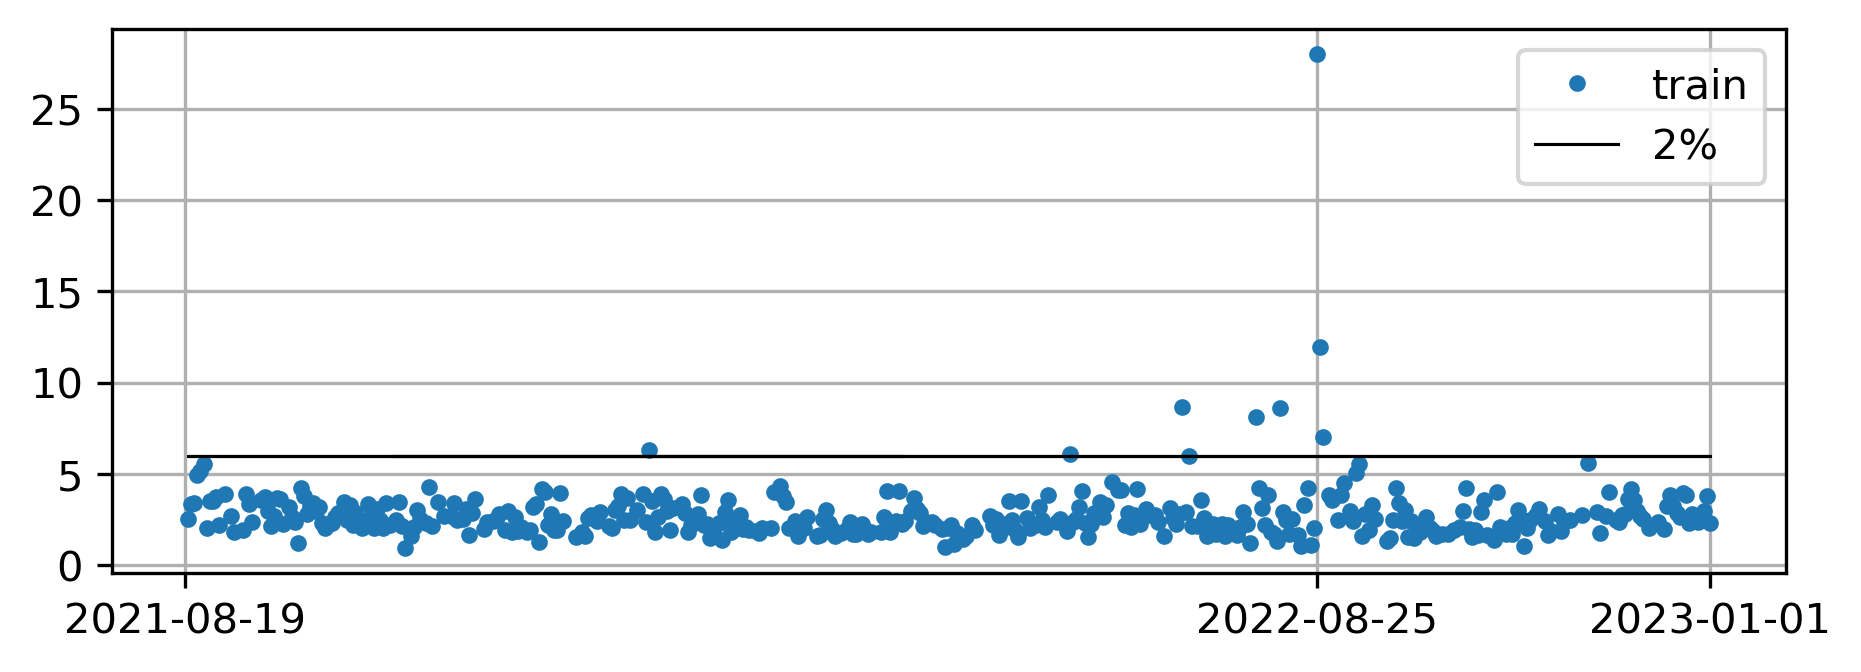
\includegraphics[width=0.9\linewidth]{pictures/train}
	\caption{Выбросы обучающей выборки}
\end{figure}

\noindent
На обучающей выборке алгоритм естественным образом возвращает 8 объектов (это ровно 2\% от 400 объектов обучающей выборки). А именно, алгоритм рекомендует детектировать как обладающие нетипичными признаками следующие даты:

\medskip
\noindent
2022-07-12, 2022-01-18, 2022-06-05, 2022-08-13, 2022-08-05, 2022-08-25, 2022-08-27, 2022-08-26.

\medskip
\noindent
Затем мы применяем алгоритм к тестовой выборке для того, чтобы исключить нетипичные объекты из пула объектов, для работы прогнозирующей модели, так как на нетипичных объектах (читай — выбросах) модель заведомо будет давать нелепый прогноз, в силу того, что обучалась на типичных данных.

\begin{figure}[!h]
	\centering
	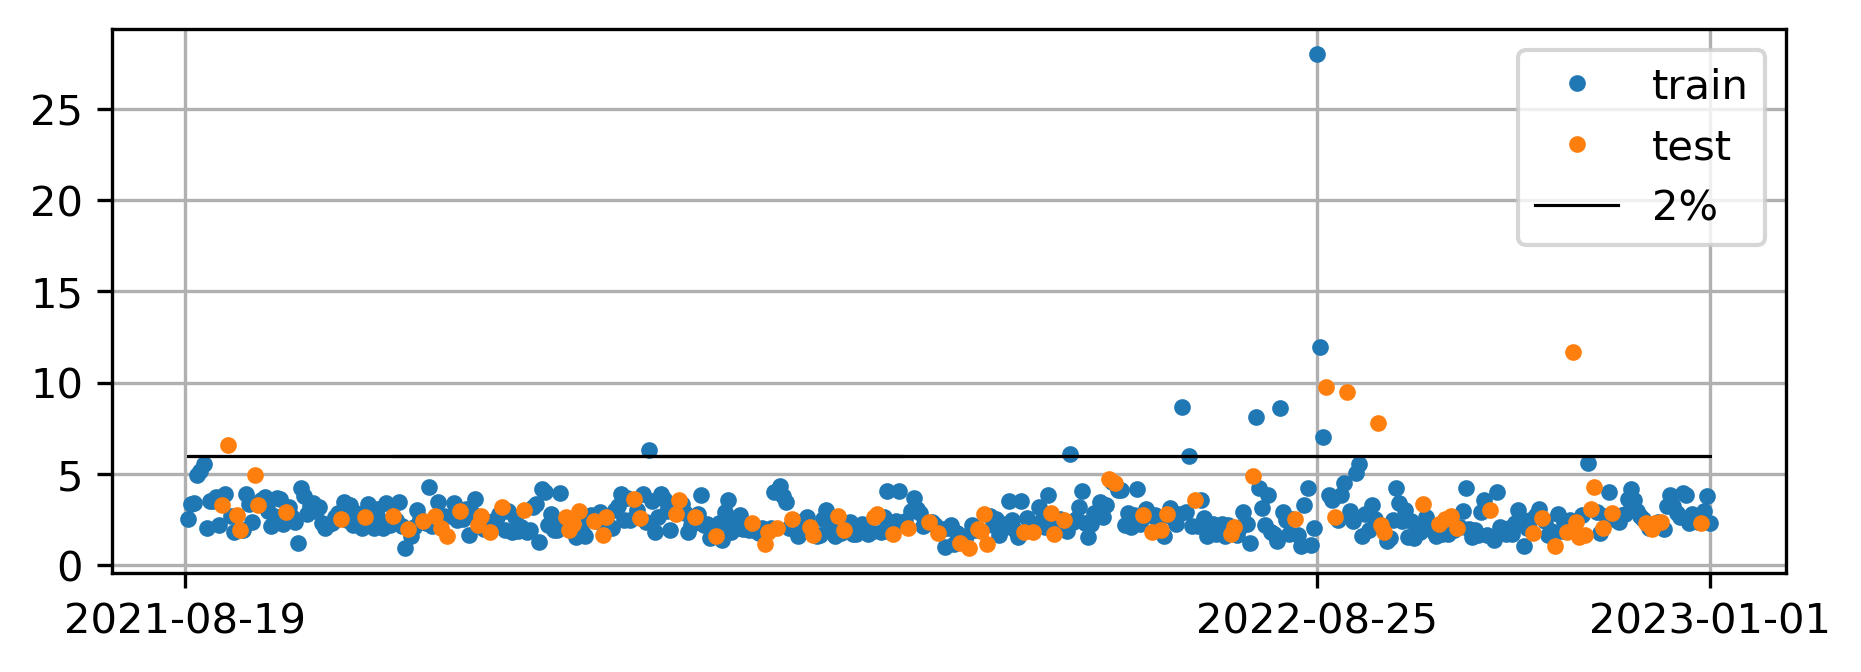
\includegraphics[width=0.9\linewidth]{pictures/test}
	\caption{Выбросы тестовой выборки}
\end{figure}
Это больше, чем 2\% от 100 объектов. Тем не менее, хорошо видно, что эти объекты действительно далеко отстоят от остальных дат по величине своих реконструкционных ошибок. В силу настройки, полученной на обучающей выборке (была настроена высота горизонтальной линии отсечения), это действительно выбросы.


\section{Выводы}

Обнаружение выбросов обычно рассматривается как задача бинарной классификации, особенно когда исследователя интересует лишь определение, является ли точка выбросом или нет. В этом случае выбросы рассматриваются как класс «положительных» или аномальных точек, в то время как все остальные точки будут принадлежать классу «отрицательных» или не-выбросов. Для решения этой задачи используются различные алгоритмы машинного обучения для бинарной классификации, такие как логистическая регрессия, случайный лес, градиентный бустинг и так далее (см. [5]).

Однако в ситуации, когда изначальная разметка данных на нормальные и аномальные объекты отсутствует, классификация невозможна. Тогда необходимы другие методы, один из которых был рассмотрен в настоящей статье и показал на примере данных о потреблении контента одного из ведущих хостингов весьма неплохие результаты. Разумеется, этот метод не является единственным в своем роде, но важно отметить, что обнаружение выбросов является субъективной задачей, и разные методы могут давать разные результаты. Поэтому всегда следует использовать комбинацию различных методов и подходов для достижения наилучших результатов.

\section{Литература}

\begin{enumerate}
	\item 1.Хейдт М. Изучаем Pandas / М. Хейдт;  — Москва: ДМК Пресс, 2018. — 438 с.
	\item Бурков А. Машинное обучение без лишних слов / А. Бурков;  — СПб: Питер, 2020. — 192 с. 
	\item Вьюгин, В. В. Математические основы теории машинного обучения и прогнозирования / В. В. Вьюгин; — М.: МЦИМО. — 2013. — 387~с. 
	\item Бринк Х. Машинное обучение / Х. Бринк, Дж. Ричардс, М. Феверолф  — СПб.: Питер, 2017. — 336 с.
	\item Дрейпер Н. Р. Прикладной регрессионный анализ / Дрейпер Н. Р., Смит Г.; ред. пер. Саит-Аметова М.; Пер. с англ. и ред. пер. Власенко М., Имамутдинова Р. Г., Орехова Н. А., Саит-Аметова М.~--- 3-е изд. --- М. : Диалектика : Вильямс, 2007. --- 911 с.
	\item Безменов И. В. Метод очистки измерительных данных от выбросов: поиск оптимального решения с минимальным количеством отбракованных результатов измерений // Измерительная техника. 2023. № 1. С. 16--23. 
	\item Безменов И. В., Дроздов А. Э., Пасынок С. Л. Стратегия поиска выбросов в рядах зашумлённых данных с неизвестным трендом // Измерительная техника. 2022. № 5. С. 29--34.
\end{enumerate}

-
\end{document}